\cotefile{136}
\scanpage{252}
\diagram{\begin{tikzcd}[ampersand replacement=\&,column sep=large]
\mathcal N=\operatorname{Mod}(k) \arrow[r,"i",shift left] \& \mathcal M_0=\mathcal M^+ \arrow[l,"\unsure{\kappa|p}"',shift left]
\end{tikzcd}}
\diagram{\begin{tikzcd}[ampersand replacement=\&]
\deleted{\unsure{N|P|\mathcal N}}\arrow[r,sloped,allow upside down,"\deleted{/}" description] \& \deleted{\mathcal M_N}\& \deleted{\unsure{\mathcal M^+}}\\[-1ex]
\& \& |[draw,ellipse]|{i,p,\unsure{S|N|\mathcal N|\rho}}
\end{tikzcd}}
\[
\begin{aligned}
i(N)&=N\otimes_k S\\
\kappa(M_*)&=M_0
\end{aligned}
\]
\[
\tau_{N,0}\circ i:\mathcal N\longrightarrow\mathcal M_N
\]
a comme adjoint à droite,
\[
\kappa\circ\rho_{0N}=\kappa\circ\tau_0\circ\rho_N=\kappa\circ\rho_N
\]
\margin{\deleted{qui a comme adjoint à gauche}}

\uline{Conditions équivalentes}

a) $i_N=\tau_{N,0}\circ i$ est pl. fidèle

b) $\forall\,\deleted{\unsure{N}}P\in\operatorname{Mod}k,\quad
\deleted{\unsure{N}}P\xrightarrow{\sim}(\rho_N i_N(\deleted{\unsure{N}}P))_0$
\[
\left[\begin{aligned}
&=(\rho_N\tau_N(\deleted{\unsure{N}}P\otimes_k S))_0\\
&=(\rho_N(P\otimes_k\tau_N S))_0
\end{aligned}\right]
\]
c) $\kappa\circ\rho_N$ est un foncteur localisation

\figure{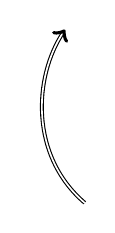
\begin{tikzpicture}[x=1cm,y=1cm]\draw[->,double] (0.4,0) .. controls (-0.3,0.6) and (-0.25,1.6) .. (0.15,2.2);\end{tikzpicture}}
\diagram{\begin{tikzcd}[ampersand replacement=\&]
\deleted{\unsure{\circ}} \& \deleted{M_0}\arrow[d] \& \deleted{M_1}\&\deleted{M_{\unsure{2|r}}\ \cdots}\\
\&\deleted{\unsure{P}}\&\&
\end{tikzcd}}
\deleted{$\unsure{\operatorname{Hom}_k(Q,P)}$}

\uline{Condition équivalente}

a$'$) \deleted{$\forall P\in\unsure{\operatorname{Mod}}$} $\operatorname{Im\,ess}i\subset\operatorname{Im\,ess}\rho_{0,N}$

b$'$) $\forall P\in\operatorname{Mod}k,$
\[
\begin{aligned}
i(P)&\xrightarrow{\sim}\rho_{0N}\tau_{N,0}\unsure{\circ i(P)|\circ(P)|i(P)}\\
&=\rho_{0N}i_N(P)
\end{aligned}
\]
b$'$\inserted{bis}) $\forall P\in\operatorname{Mod}k,\quad i(P)\xrightarrow{\unsure{\sim}}\rho_{0N}i_N(P)$ est un isom en dim $0\leq\alpha\leq N-1$

c$'$) \inserted{$\forall P\in\operatorname{Mod}k,$} $\forall\,0\leq\alpha\leq N-1,$ \deleted{$\tau_{N-\alpha,0}S$} on a
\diagram{\begin{tikzcd}[ampersand replacement=\&,row sep=small]
P\otimes_k S_\alpha \arrow[r,"\sim"] \& \operatorname{Hom}^{\alpha}(\tau_{N-\alpha}S,\deleted{\unsure{Q}}P\otimes_k S)\\
\bigl[\operatorname{Hom}^{\alpha}(S,P\otimes_k S)\bigr] \arrow[u,"\wr"'] \arrow[ur,dashed,"\text{\unsure{restrict.|restriction}}"' ] \&
\end{tikzcd}}
\[
\operatorname{Hom}^{\alpha}(S/\tau_{N-\alpha}S,P\otimes_k S)=0
\]
% archive sheet number: 251

\scanpage{253}
% Manuscript upside down in the scan; references follow the upright writing.
\[
J\subset A
\]
$H^*(X,J)^{\deleted{\unsure{*}}}$ à p.d.
% A long diagonal stroke begins to the left of the following presentation.
\[
\begin{aligned}
A\{(X_i)_{i\in I},(Y_i)_{i\in I}\}/\bigl(&\textstyle\sum X_i-\pi,\sum Y_i-\omega,\sum dX_i,\\
&\textstyle\sum dY_i\bigr)
\end{aligned}
\]
\[
\overset{\unsure{\sim|-|\rightarrow}}{\deleted{A}\quad A^{(I)}}
\]
\figure{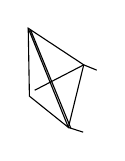
\begin{tikzpicture}[scale=.75]\draw (0,1.6)--(.94,.98)--(.68,-.08)--(.02,.45)--cycle;\draw (0,1.6)--(.68,-.08) (.04,1.57)--(.72,-.09) (.11,.55)--(.94,.98); \draw (.94,.98)--(1.16,.89) (.68,-.08)--(.93,-.16);\end{tikzpicture}}
\deleted{\[
\begin{aligned}
&\Gamma^*_{(A,\pi)}(A^I\otimes_A J)\\
&X_{\unsure{1|i}}\otimes\pi,\ X_{\unsure{2}}\otimes\pi,\ -,\ X_{\unsure{m|n}}\otimes\pi\\
&\textstyle\sum X_i\otimes\pi-\pi\\
&\deleted{J^I/J}\\
&\Gamma^*_{(A,J)}(J^I)/\delta J\\
&\delta\pi=\deleted{\unsure{\pi}}-\pi+\pi
\end{aligned}
\]}
$\unsure{K|L|\Gamma}_A^*.$
\deleted{\[
A\bigl\{(X_i)_{i\in I}\inserted{dX_i}\bigr\}/\bigl(\sum_{\unsure{I}}\pi X_i-\pi\,;\ \pi\sum dX_i\bigr\}
\]}
\[
\Gamma_A^{*+}J\longrightarrow J
\]
\[
H^*(X,\Gamma^{\alpha+}J)\longrightarrow H^\alpha(X,J)
\]
\deleted{\diagram{\begin{tikzcd}[ampersand replacement=\&]
\&\& H^{\unsure{2\alpha|2i\alpha}}(X,\operatorname{Sym}^{\alpha}M)\\
H^{2i}(X,M)\arrow[r,"\gamma^\alpha"] \& H^{2i\alpha}(X,\Gamma^\alpha M)\arrow[ur] \&
\end{tikzcd}}
\[
H^{2i}(X,J)\longrightarrow H^{2i\alpha}(X,\Gamma^\alpha J)\longrightarrow H^{2i\alpha}(X,J)
\]}
\diagram{\begin{tikzcd}[ampersand replacement=\&]
A\arrow[r,"2i"]\arrow[dr,"2i\alpha"'] \& M\\
\&\Gamma^\alpha M
\end{tikzcd}}
\diagram{\begin{tikzcd}[ampersand replacement=\&]
\Gamma^i M\arrow[d,shift right] \& x^{(i)}\arrow[d,mapsto]\& \substack{i!x^{(i)}\\ \Vert\\ x^i}\\
\operatorname{Sym}^i(M)\arrow[u,shift right]\&x^i\&\unsure{x}\arrow[u]
\end{tikzcd}}
% archive sheet number: 252

\scanpage{254}
\[
\mathcal M/\operatorname{Neg}_{\infty}\simeq\underset{\longrightarrow}{\operatorname{Lim}}\,\mathcal M_N
\]
n'est pas une catégorie à \uline{$\operatorname{lim}$} filtrantes exactes.
% archive sheet number: 253

\scanpage{255}
% letterhead
UNIVERSITE DES SCIENCES ET TECHNIQUES\\
DU LANGUEDOC

MATHEMATIQUES\hfill Montpellier, le 16 Juin 1975

SEMINAIRE D'ANALYSE CONVEXE

Jeudi 19 juin 1975, à 11 h, Salle 431

Mr A. BENSOUSSAN - Professeur, Université Paris IX Dauphine.

Diffusions réfléchies.
% archive sheet number: 254

\scanpage{256}
$S$-module $N$-négligeable $M$ \quad $(N\in\mathbb Z)$
\[
\overset{\mathrm{def}}{\Longleftrightarrow}\tau_N M=0
\Longleftrightarrow M_i=0\quad\text{si }i\geq N
\]

module $\infty$-négligeable $M$
\[
\begin{aligned}
&\Longleftrightarrow \exists\,N\in\mathbb Z\ \text{tel que }M\ \text{$N$-\unsure{négl.|négligeable}}\\
&\Longleftrightarrow M_i=0\quad\text{si }i\text{ assez grand}
\end{aligned}
\]

\uline{Rmq} Si $M$ de type fini, $M$ est
\[
\left|\begin{aligned}
&\infty\text{-négligeable ssi }\exists\,N\unsure{\geq|\gg}0\\
&\text{tel que }\tau_N S\text{ annule }M
\end{aligned}\right.
\]

$M$ négligeable $\Longleftrightarrow M$ limite inductive de modules $\infty$ négligeables

$\Longleftrightarrow$ tt sous-module de t.f. de $M$ est $\infty$-négligeable

$\Longleftrightarrow\forall x\in M,\ \exists\,N\geq 0$ tel que $\tau_N S$ annule $x$

\[
\begin{gathered}
\operatorname{Nég}_N\subset\operatorname{Nég}_{N'}\subset\operatorname{Nég}_\infty\subset\operatorname{Nég}\\
N\leq N'
\end{gathered}
\]
$\operatorname{Nég}_N,\operatorname{Nég}_\infty$ sous-catégories épaisses de $\mathcal M$,
\diagram{\begin{tikzcd}[ampersand replacement=\&]
\mathcal M/\operatorname{\unsure{Nêg|Nég}}_N\arrow[d]\arrow[r,phantom,"\simeq"]\&\mathcal M_N\arrow[d,"\tau_{N',N}"]\\
\mathcal M/\operatorname{Nég}_{N'}\arrow[r]\&\mathcal M_{N'}
\end{tikzcd}}
% archive sheet number: 255

\scanpage{257}
\[
\varinjlim\,\unsure{\varphi|\rho}_N\tau_N P\longrightarrow\varphi_\infty\tau_\infty P
\]
\deleted{Hom}\quad bijectif ?
\[
\Downarrow
\]
$\forall M$ de \unsure{prés|prés.} finie (il suffit $M=S[i]$)
\diagram{\begin{tikzcd}[ampersand replacement=\&,column sep=small,execute at end picture={\draw ([xshift=-2pt]\tikzcdmatrixname-2-2.west |- \tikzcdmatrixname-2-2.north) -- ([xshift=-2pt]\tikzcdmatrixname-2-2.west |- \tikzcdmatrixname-4-1.south);}]
\operatorname{Hom}_{\mathcal M}(M,\underset{\unsure{\rightarrow|-}}{\lim}\varphi_N\tau_N P)\arrow[r,dash]\arrow[d,phantom,"\rotatebox{90}{$\simeq$}"] \& \operatorname{Hom}_{\mathcal M}(M,\varphi_\infty\tau_\infty P)\quad\text{bij}\arrow[d,phantom,"\rotatebox{90}{$\simeq$}"]\\
\varinjlim\operatorname{Hom}_{\mathcal M}(M,\deleted{\unsure{\tau}}\varphi_N\tau_N P)\arrow[d,phantom,"\rotatebox{90}{$\simeq$}"] \&\operatorname{Hom}_{\mathcal M_\infty}(\tau_\infty M,\tau_\infty P)\arrow[d,phantom,"\rotatebox{90}{$\simeq$}"]\\
\varinjlim\operatorname{Hom}_{\mathcal M_N}(\tau_N M,\tau_N P)\arrow[d,phantom,"\rotatebox{90}{$\simeq$}"] \& \underset{\substack{\longrightarrow\\ M'\subset M\\M/M'\ \text{négl.}}}{\lim}\operatorname{Hom}(M',P)\\
\underset{\unsure{-|\rightarrow}}{\lim}\operatorname{Hom}_{\mathcal M}(\tau_N M,P)\arrow[ur]\&
\end{tikzcd}}

dire que (pour $M$ fixé) c'est un isom pour tt $P$, signifie que les sous pro-objets de $M$ \unsure{formés}, soit des $\tau_N M$, soit des $M'\subset M$ tels que $M/M'$ soit négligeable, \deleted{\unsure{sont|soit}} isom par l'hom can., ou encore que, \unsure{ces ens|ces deux} de sous-objets sont cofinaux, i.e que tout $M'$ contient un $\tau_N M$ \inserted{i.e $M/M'$ est $\infty$-négligeable.}

Mais c'est le cas si $M$ de \deleted{\unsure{prés.}}\inserted{t.f.}

\deleted{\uline{Hyp} Tout idéal gradué $J$ de $S$, tel que $S/J$ soit négligeable}

\deleted{\unsure{finité}.} Donc
\[
\varinjlim\,\varphi_N\tau_N P\xrightarrow{\sim}\varphi_\infty\tau_\infty P
\]
% archive sheet number: 256

\scanpage{258}
% letterhead
U N I V E R S I T E\hfill Montpellier, le 24 juin 1975\\
DES SCIENCES ET TECHNIQUES\\
\uline{DU LANGUEDOC}\\
AMC/MD

\uline{Diffusion} : Liste A\\
n° 4135

% printed form
AVIS DE SOUTENANCE D'UNE THESE DE DOCTORAT DE

\uline{SPECIALITE : CHIMIE}

Mention Chimie Organique Physique

\uline{Nom et prénom du candidat} : DALVERNY Gilbert

\uline{Titre de la thèse} : Synthèse et réactivité d'organomagnésiens perfluorés. Application à la préparation d'acides perfluorosulfoniques et carboxyliques.

\uline{Date, heure et lieu de soutenance prévus} : 10 juillet 1975 à 11 heures, salle de cours n° 9 - U.S.T.L.

\uline{Nom du Directeur de thèse} : Monsieur le Professeur A. COMMEYRAS

\uline{Désignation du laboratoire où la thèse est préparée} : Laboratoire de chimie organique

\uline{Analyse de l'ouvrage} : Des méthodes de synthèses, par voie chimique, d'acides perfluoroalcanesulfoniques $\mathrm{R_FSO_3H}$ et carboxyliques $\mathrm{R_FCO_2H}$ ont été mises au point ; elles font intervenir comme intermédiaires réactionnels, les organomagnésiens perfluorés saturés $\mathrm{R_FMgX}$ correspondants.

Des possibilités d'application de la réaction magnésienne au niveau de composés perfluorés insaturés ont été ensuite étudiées.

\uline{Durée approximative des recherches ayant abouti à la thèse} : 2 ans

\uline{Composition du jury proposé} : M. A. COMMEYRAS - Président\\
M. R. CORRIU\\
M. A. CAMBON\\
M. R. MARTIN

Le Secrétaire Général,\\
\figure{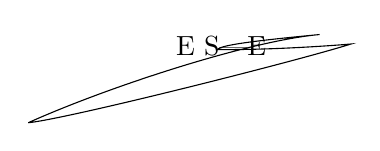
\begin{tikzpicture}[x=1cm,y=1cm]\draw (0,0) .. controls (1,.45) and (2.8,1.04) .. (3.7,1.12) .. controls (2.75,1.03) and (2.45,.98) .. (2.4,.93) .. controls (3.1,.92) and (4,.99) .. (4.1,1) .. controls (3.4,.78) and (.5,.05) .. (0,0);\node at (2.45,.97) {\handwritten{\unsure{E S|E}}};\end{tikzpicture}}
\uline{E. SIAU}
% archive sheet number: 257

\scanpage{259}
\[
\begin{aligned}
(\unsure{\varphi|\rho}_\infty\tau_\infty P)_{i}
 &\simeq\operatorname{Hom}^i(S,\varphi_\infty\tau_\infty P)\\
 &\simeq\operatorname{Hom}(S[-i],\varphi_\infty\tau_\infty P)\\
 &\simeq\operatorname{Hom}(\tau_\infty S[-i],\tau_\infty P)\\
 &\simeq\underset{\substack{\longrightarrow\\M'\subset S[-i]\\\text{t.q. }S[\unsure{i|-i}]/M'\ \text{négl.}}}{\lim}
 \deleted{\unsure{f|\operatorname{Hom}}}\operatorname{Hom}(M',P)\\
 &\simeq\underset{\substack{\unsure{\rightarrow|-}\\M'\subset S\\\text{t.q. } S/M'\ \text{négl.}}}{\lim}\operatorname{Hom}^i(M',P)\\
 &\simeq\underset{\substack{\longrightarrow\\N}}{\lim}
 \underbrace{\operatorname{Hom}^i(\tau_N S,P)}_{\substack{\rotatebox{90}{$\simeq$}\\\operatorname{Hom}^i(\tau_N S,\tau_{N+i}P)}}\\
 &\simeq\underset{\substack{\unsure{-|\rightarrow}\\N}}{\lim}\operatorname{Hom}(\tau_N(S[-i]),\tau_N P).
\end{aligned}
\]

\figure{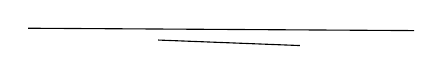
\begin{tikzpicture}[x=1cm,y=1cm]\draw (0,0)--(4.9,-.03) (1.65,-.15)--(3.45,-.22);\end{tikzpicture}}
\diagram{\begin{tikzcd}[ampersand replacement=\&]
\tau_N S\arrow[r,"d^\circ\,0"]\arrow[d,"{\cdot T^{(\ell)}}"']\&P\\
\tau_{N+\ell}(S)\arrow[ur,"{d^\circ\,\deleted{\unsure{0}} \unsure{(\ell)|-\ell|\ell}}"]\&
\end{tikzcd}}
\[
\unsure{\xi|\zeta|\sum}T^{(i)}\overset{T^{(\ell)}}{\longmapsto}\xi c_{i,\ell}T^{(i+\ell)}
\]

\figure{\begin{tikzpicture}[scale=.4]\draw (1,3.7)--(3.6,0) (3.5,-.1)--(0,-3.1)--(-.03,-4);\end{tikzpicture}}
\[
\begin{gathered}
P\in\operatorname{Im\,ess}\varphi_\infty\\
\Updownarrow\\
P\xrightarrow{\sim}\varphi_\infty\tau_\infty P\\
\Updownarrow\\
\operatorname{Hom}^i(S,P)\xrightarrow{\sim}\underset{\substack{\longrightarrow\\N}}{\lim}\operatorname{Hom}^i(\tau_N S,P)
\end{gathered}
\]
a) \uline{injectivité} : $P$ n'a pas d'élément négligeable non nul

b) surjectivité : tout homom. \inserted{homog} d'un \deleted{\unsure{degré}} $\tau_N S$ ds $P$ se prolonge à $S$, ou encore :

toute ext. de $[S/\tau_N S][-i]$ par $P$ est triviale \ldots
% archive sheet number: 258

\scanpage{260}
\mspage{- 99 -}\hfill IX

que l'on a une \uline{immersion ouverte} canonique
\[
A^{\handwritten{\natural}}_{K,K'}\handwritten{\hookrightarrow}A^{\handwritten{\natural}}_{K,K''}\ ,\tag*{(8.3.1)}
\]
permettant d'identifier le premier groupe à un sous-groupe ouvert du deuxième. Pour $K'$ variable, on voit que les $A_{K,K'}$ forment ainsi un système inductif de groupes lisses de type fini sur $K$, à morphismes de transition des immersions ouvertes. Si on pose
\[
\Phi_{K,K'}=A^{\handwritten{\natural}}_{K,K'}/A^{\handwritten{\natural}\,\unsure{o|0|\circ}}_{K,K'}\ ,\tag*{(8.3.2)}
\]
les $\Phi_{K,K'}$ eux-mêmes forment donc un système inductif de groupes finis étales sur $K$, qui sera étudié plus en détail plus bas.

Nous poserons
\[
A^{\handwritten{\unsure{\flat|b}}}_K=\underset{K'}{\mathop{\lim}\limits_{\handwritten{\longrightarrow}}}A^{\handwritten{\natural}}_{K,K'}\ ,\tag*{(8.3.3)}
\]
la limite étant prise dans la catégorie des faisceaux fppf sur $K$. Comme les morphismes de transition dans le système inductif envisagé dans des immersions ouvertes, il est d'ailleurs clair que cette limite est en fait représentable par un schéma en groupes (en général non quasi-compact) sur $K$, que nous désignerons comme de \unsure{juste|juśte} par le même \unsure{symbole|symbôle} $A^{\handwritten{\flat}}_K$. On notera qu'on a, pour ce schéma en groupes
\[
A_K^{\handwritten{\flat}\,o}=A_K^{\handwritten{\natural}\,o}\ ,\
A_K^{\handwritten{\flat}}/A_K^{\handwritten{\flat}\,o}\ \simeq\
\underset{K'}{\mathop{\lim}\limits_{\handwritten{\longrightarrow}}}\Phi_{K,K'}\ .\tag*{(8.3.4)}
\]
Ce dernier groupe sera déterminé dans 11.10 : il est canoniquement isomorphe à $\underline{M}_K\otimes\mathbb Q/\mathbb Z$ (avec la notation (8.1.8)).

\handwritten{417}
\mspage{417}
% archive sheet number: 259

\scanpage{261}
\[
\operatorname{Hom}_{\mathcal M}(M,\unsure{\varphi|\rho}_N\deleted{\tau_N}\underset{\substack{\rotatebox{90}{$\in$}\\\mathcal M_N}}{P})\simeq
\operatorname{Hom}_{\mathcal M_N}(\tau_N M,\deleted{\tau_N}P)
\]
donc
\[
\begin{aligned}
(\varphi_N\tau_N P)_i&=\operatorname{Hom}_{\mathcal M}^i(S,\varphi_N\tau_N P)=\operatorname{Hom}_{\mathcal M}(S[-i],\varphi_N\deleted{\tau_N}P)\\
&=\operatorname{Hom}_{\mathcal M_N}(\tau_N(S[-i]),\deleted{\tau_N}P)\\
&\simeq\operatorname{Hom}_{\mathcal M_N}((\tau_{N-i}(S))(-i),\deleted{\tau_N}P)\\
&\simeq\operatorname{Hom}_{\mathcal M}^i(\tau_{N-i}(S),\deleted{\tau_N}P)
\end{aligned}
\]

\noindent\rule{.91\linewidth}{.3pt}\par
$h_M=\operatorname{Hom}(M,-)$, donc $h_M\circ\varphi_N\deleted{\circ\tau_N}\simeq h_{\tau_N M}\deleted{\circ\tau_N}$

\deleted{donc $h_M\circ\varphi_N\circ\tau_N\simeq h_{\tau_N M}\circ\tau_N$}

\deleted{$R^*(h_M\circ\varphi_N\tau_N)\simeq R^{\alpha}h_{\tau_{\unsure{\cdot}}}$}

Composons avec $\tau_N$, on a
\[
\begin{aligned}
\operatorname{Hom}_{\mathcal M}(M,\rho_N\tau_N P)&=\operatorname{Hom}_{\mathcal M_N}(\tau_N M,\tau_N P)\\
&\simeq\operatorname{Hom}_{\mathcal M}(i_N\tau_N M,P)
\end{aligned}
\]
\[
h_M\varphi_N\tau_N=h_{i_N\tau_N}
\]
D'où
\[
\begin{aligned}
R^*(h_M\varphi_N\tau_N)&\simeq R^{\alpha}h_{i_N\tau_N}=\unsure{\mathbb R|R}\operatorname{Hom}(i_N\tau_N M,-)\\
\rotatebox{90}{$=$}&\\[-1ex]
\deleted{\unsure{R}}\mathbb R^*(h_M\varphi_N)&\underbrace{\tau_N}_{\substack{\rotatebox{90}{$=$}\\R^\alpha\tau_N\ \text{car }\tau_N\ \text{exact}}}
\end{aligned}
\]
Si $M$ \uline{projectif} donc $h_M$ exact, on aura
\[
h_M\cdot(R^*\varphi_N)\circ\tau_N\simeq\mathbb R\operatorname{Hom}(\tau_N M,-)
\]
i.e.
\[
\deleted{\unsure{\mathbb R}}\boxed{\operatorname{Hom}(M,R^*\varphi_N(\tau_N P))\simeq\mathbb R\operatorname{Hom}(\tau_N M,P)}
\]
en particulier :
\[
\deleted{\operatorname{Ext}}\quad
\boxed{\begin{gathered}
\operatorname{Hom}(M,(R^{\unsure{k|n}}\varphi_N)(\tau_N P))\simeq\deleted{\unsure{R}}\operatorname{Ext}^{k}(\tau_N M,P)\\
\text{si } M\ \text{projectif }\in\deleted{\unsure{D}}\mathcal M
\end{gathered}}
\]
% archive sheet number: 260

\scanpage{262}
\mspage{- 94 -}\hfill IX

la biextension $W^{\mathrm{ab}}$ de $(B,B')$ par $\mathbb G_{mS}$ est une dualité parfaite sur $U$ (ou ce qui revient au même si $U$ est dense dans $S$, sur $\unsure{S}$). C'est une propriété qu'il suffit de vérifier en tout point $\eta$ de $\unsure{U}$, et alors l'argument habituel nous ramène au cas où $S$ est un \unsure{trait} de point générique $\eta$, qui est déjà connu.

La relation d'orthogonalité nous permet d'autre part d'étendre au cas présent les formules (5.5.7), (5.5.8) et (5.5.9), où on remplace l'opération de restriction au point générique $\eta$ par celle de restriction à l'ouvert $U$ ; par suite, 5.6 s'étend également au cas présent. Nous nous dispensons de réécrire ici les formules et l'énoncé précédents dans le contexte présent.

Résumons, du point de vue des modèles de Néron, les résultats obtenus concernant les parties abéliennes et leurs accouplements :

\uline{Proposition} 7.5. \uline{Soit} $S$ \uline{un trait complet}, \uline{de corps de fonctions} $K$. A \uline{tout schéma abélien} $A_K$ \uline{sur} $K$ \uline{ayant une réduction semi-stable sur} $S$, \uline{le procédé de} 7.1, \uline{appliqué à la composante neutre du modèle de Néron} $A$, \uline{de} $A_K$ \uline{permet de définir la} partie abélienne $B=A^{\mathrm{ab}}$ \uline{de celui-ci}, \uline{qui est un schéma abélien sur} $S$, \uline{dépendant fonctoriellement de} $A_K$. \uline{Pour tout autre schéma abélien} $A'_K$ \uline{à réduction semi-stable}, \uline{on peut à toute correspondance divisorielle} $W_K$ \uline{sur} $(A_K,A'_K)$, \uline{associer une correspondance divisorielle unique} $W^{\mathrm{ab}}$ \uline{sur} $(A^{\mathrm{ab}},A'^{\mathrm{ab}})$, \uline{telle que pour tout entier} $n\geq 0$, $W_n^{\mathrm{ab}}$ \uline{ait comme image inverse par} $A_n^{\unsure{o|0|\circ}}\handwritten{\longrightarrow} B_n=A_n^{o\mathrm{ab}}$, $A'_n{}^o\handwritten{\longrightarrow} B'_n=A'_n{}^{o\mathrm{ab}}$ \uline{la biextension} $W_n$ \uline{de} $(A_n^o,A'_n{}^o)$ \uline{déduite de} $W$ \uline{par réduction}, \uline{où} $W$ \uline{est le prolongement canonique} (1.4) \uline{de} $W_K$ \uline{à} $(A^o,A'{}^o)$.

\handwritten{412}
\mspage{412}
% archive sheet number: 261

\scanpage{263}
\uline{Ex} \quad $M=S[-i]$, on \unsure{trouve}
\[
\begin{aligned}
\unsure{\kappa|k|H}_i(R^*\unsure{\varphi|\rho}_N(\tau_N(P))&\simeq\mathbb R\operatorname{Hom}(\tau_N(S[-i]),P)\\
&\simeq\mathbb R\operatorname{Hom}((\tau_{N-i}S)[-i],P)\\
&\simeq R\operatorname{Hom}^i(\tau_{N-i}S,P).
\end{aligned}
\]
donc
\[
(R^n\varphi_N(\tau_N P))_i=\mathbb E\mathrm{xt}^n((\tau_{N-i}S)[-i],P)
\]
\uline{NB} C'est valable aussi en remplaçant $\varphi_N$ par $\varphi_{N',N}$ $(N'\leq N)$ pourvu que $i\geq N'$ (si $i<N'$, on trouve 0 bien sûr !)

\deleted{\uline{NB} Supposons $P\in\operatorname{Im\,ess}\varphi_{N',N}$ \quad $(N'\leq N)$

i.e. $\deleted{\unsure{\varphi_{N'}}}P\xrightarrow{\sim}\varphi_{N',N}\tau_N P=R^0\varphi_{N',N}(\tau_N P)$

Alors $R^n(\varphi_{N',N}(\tau_N P))=0$ si $n>0$

i.e. $\operatorname{Ext}^n(\tau_{N-i}(S)[-i],P)=0$ si $\substack{i\geq N'\\ n>0}$

En effet, cela revient à}

\deleted{\[
R^{\unsure{n|*}}\unsure{\varphi_N}\varphi_N\unsure{\tau(P)}_{\substack{\rotatebox{90}{$\in$}\\\mathcal M_N}}
\]}

Soit $C$ une catégorie abélienne, \inserted{$\unsure{N'_0|N_0^*|N_0}\leq N$ ds $\mathbb Z$} et
\[
C\xrightarrow{i}\mathcal M_{\unsure{N_0|N'_0}}
\]
un foncteur \uline{exact}, tel que
\[
i(C)\subset\operatorname{Im\,ess}\varphi_{N'_0,N}
\]
i.e
\[
i(\unsure{\deleted{M}|\underline M|M})\xrightarrow{\sim}\varphi_{N'_0,N}\tau_{N,N'_0}i(M)
\]
Je dis qu'alors
\[
(R^n\varphi_{N'_0,N})(\tau_{N,N'_0}\circ i)=0\quad\text{si }n>0
\]
En effet, comme $i\simeq\varphi_{N'_0,N}\tau_{N,N'_0}i$ on en déduit
\diagram{\begin{tikzcd}[ampersand replacement=\&,column sep=small]
R^\alpha i\arrow[d,phantom,"\rotatebox{90}{$\simeq$}"] \& {}\simeq R^\alpha(\varphi_{N'_0,N}\tau_{N,N'_0})\arrow[d,phantom,"\rotatebox{90}{$\simeq$}"]\\
i\quad\text{car }i\text{ exact}\& (R^*\varphi_{N'_0,N})(\tau_{N,N'_0}\circ i)\quad\text{car }\tau_{N,N'_0}\text{ est exact}
\end{tikzcd}}
% archive sheet number: 262

\scanpage{264}
\mspage{- 76 -}\hfill IX

de prolonger ce groupe de Barsotti-Tate en un sous-groupe de Barsotti-Tate $F$ de $A$, qui jouerait alors le rôle joué par la \uline{partie fixe} $T_{\handwritten{\ell}}(A)^f$ de (\unsure{2,2.3.2|2.2.3.2}) dans le cas où $A^{\unsure{o|0|\circ}}$ est $\handwritten{\ell}$-divisible. Dans le cas semi-stable, où on a $\overline A_{\unsure{o|0}}=A_o^o$,la question se résoud par l'affirmative par la méthode de 2.2. Dans le cas général, lorsque le problème envisagé a une solution, on voit facilement qu'elle est unique, et que les sous-pro-groupes correspondants de $T_p(A_K)$ et de $T_p(A'_K)$ (qui méritent alors encore le nom de \uline{partie fixe} des pro-groupes envisagés) satisfont encore au théorème d'orthogonalité 5.2, enfin que la partie fixe $T_p(A_K)^f$ peut encore se caractériser comme indiqué dans 5.8.

6.2.1. Montrons cependant qu'en général le problème envisagé n'a pas une solution affirmative, i.e. qu'\uline{il n'est pas possible en général de définir la partie fixe} $T_p(A)^f$ (cas de la réduction non semi-stable). En effet, en vertu d'un théorème de relèvement de SERRE-TATE [30], lorsque $S$ est complet, l'existence de la partie fixe équivaut à celle de relèvements infinitésimaux $\overline A_n$ de $\overline A_o$ dans les $A_n$, ou encore à celle d'un schéma en groupes lisse $\bar A$ sur $S$, extension d'un schéma abélien par un tore $T$, de fibre spéciale $\overline A_o$, et d'un homomorphisme formel $\widehat{\bar A}\handwritten{\longrightarrow}\unsure{\widehat A|\dot A}$ prolongeant l'inclusion sur les fibres spéciales. Donc, dans le cas où $\overline A_o$ est un schéma abélien i.e. où $T_o=0$, cela équivaut à l'existence d'un schéma abélien $\bar A$ prolongeant $\overline A_o$ et d'un homomorphisme $\bar A\handwritten{\longrightarrow} A$ prolongeant l'inclusion des fibres spéciales. Il suffira donc de donner un cas où $T_o=0$, où $A_o^o$ est non unipotent et non propre, et où $A_K$ est simple sur $K$.

\handwritten{394}
\mspage{394}
% archive sheet number: 263

\scanpage{265}
d'où la conclusion

Le cas qui nous intéresse est
\[
N_0=0\leq N,\qquad C=\operatorname{Mod}(k),
\]
$i(M)=M\otimes_k S$, et où on sait que
\[
M\otimes_k S\subset\operatorname{Im\,ess}\unsure{\varphi|\rho}_{0N}\qquad\forall M\in\operatorname{Mod}(k)
\]
i.e.
\[
M\otimes_k S\simeq\varphi_{0N}\tau_N(M\otimes_k S)\quad(=R^0\varphi_{0N}(\tau_N M\otimes_k S))
\]
\deleted{\[
\begin{gathered}
\rotatebox{90}{$=$}\\
\operatorname{Hom}((\tau_{N-i}S)[-i],M\otimes_{\unsure{k|r}}
\end{gathered}
\]}
alors on a
\[
R^n\varphi_{0N}(\tau_N(M\otimes_k S))=0\quad\text{si }n>0
\]
i.e.
\[
\boxed{\begin{aligned}
&\operatorname{Ext}_{\mathcal M}^n((\tau_{N-i}S)[-i],M\otimes_k S)=0\quad\text{si}\\
&\hfill n>0,\ i\geq 0
\end{aligned}}
\]

\noindent\rule{.98\linewidth}{.3pt}\par
\[
\operatorname{Hom}_{\mathcal M}(M,\varphi_\infty\tau_\infty P)\simeq\unsure{\ldots}\underset{\inserted{\text{si }M\text{ de prés. finie}}}{\simeq}
\underset{\substack{\rightarrow\\N}}{\lim}\operatorname{Hom}_{\mathcal M}^{\deleted{\unsure{*}}}(\tau_{N\deleted{\unsure{-i}}}M,\deleted{\unsure{\tau}}P)
\]
Si de plus $M$ projectif
\[
\operatorname{Hom}(M,R^*\varphi_\infty(\tau_\infty P))\simeq
\underset{\substack{\longrightarrow\\N}}{\lim}R\operatorname{Hom}_{\mathcal M}((\tau_{N\deleted{\unsure{-i}}}M)\deleted{[\unsure{-i}]},-)
\]
en particulier
\[
\operatorname{Hom}(M,R^{\unsure{n}}\varphi_\infty P)\simeq
\underset{\substack{\longrightarrow\\N}}{\lim}\operatorname{Ext}^{\unsure{n}}_{\mathcal M}((\tau_{N-i}M)[-i],P)
\]
p.ex. si $\deleted{S}M=S[i]$, on \unsure{trouve}
\[
\begin{aligned}
\deleted{\unsure{R^*}}(\varphi_\infty\tau_\infty P)_i
 &=\underset{\substack{\longrightarrow\\N}}{\lim}\operatorname{Hom}^i(\tau_{N-i}S,P)\\
(R^\alpha\varphi_\infty(\tau_\infty P))_{\unsure{j|i}}
 &\simeq\underset{\substack{\longrightarrow\\N}}{\lim}R^\alpha\operatorname{Hom}^i\deleted{\unsure{(}}(\tau_{N-i}(S),P)\\
\deleted{\unsure{\operatorname{Ext}^i}}(R^n\varphi_\infty(\tau_\infty P))_i
 &\simeq\underset{\substack{\longrightarrow\\N}}{\lim}\operatorname{Ext}_{\mathcal M}^n(\tau_{N-i}(S)[-i],P)
\end{aligned}
\]
% archive sheet number: 264

\scanpage{266}
\mspage{- 84 -}\hfill IX

\uline{Proposition} 7.1.5. \uline{Avec les notations précédentes pour} $S,A,\ \hat B$, \uline{supposons que} $S$ \uline{soit} normal. \uline{Alors} $\hat B$ \uline{est algébrisable}, \uline{et le schéma abélien} $B$ \uline{sur} $S$ \uline{dont il provient est projectif sur} $S$.

On peut évidemment supposer $A=A^{\unsure{o|0|\circ}}$, et $S$ intègre. D'après M. RAYNAUD [23 XI 1.13], l'hypothèse que $S$ est normal implique que $A$ est quasi-projectif sur $S$. Soit donc $\underline L$ un Module inversible sur $A$ qui est relativement ample, et formons le Module birigidifié $\delta(\underline L)=\pi^*(\underline L)\operatorname{pr}_1^*(\underline L)^{-1}\operatorname{pr}_2^*(\underline L)^{-1}$ sur $A\times_S A$ comme dans VIII 4.12. Comme les fibres de $A_{\unsure{o|0}}$ sont de rang unipotent nul, il en est de même de celles de $A$ (résulte facilement de 3.1), donc en vertu de VIII 7.5, $\delta(\underline L)$ définit une biextension $W$ de $(A,A)$, évidemment symétrique, qui en vertu de VIII 4.13 (i.e. essentiellement en vertu de RAYNAUD [23 XI 1.11]) satisfait à la condition d'amplitude voulue en les points de $S_o$.

\uline{Remarque} 7.1.6. On peut prouver, sans hypothèse de normalité sur $S$, que $\hat B$ est toujours algébrisable, en se ramenant au cas normal comme dans 13.5.3 a).

7.2. Notons maintenant le

\uline{Lemme} 7.2.1. \uline{Soient} $S$ \uline{le spectre d'un anneau noethérien} $V$, \uline{séparé et complet pour la topologie définie par un idéal} $\underline m$ \uline{de} $V$, $C$ \uline{la catégorie des schémas en groupes} $A$ \uline{sur} $S$, \uline{lisses de type fini sur} $S$, \uline{tels que} $A/A^o$ \uline{soit un schéma en groupes étale fini sur} $S$ \uline{et que} $A^o$ \uline{soit une extension d'un schéma abélien} $B$ \uline{par un tore isotrivial} $T$ (SGA 3 IX 1.1),

\handwritten{\unsure{402|407}}
\mspage{402}
% archive sheet number: 265
